\pdfminorversion=7
\documentclass[12pt,letterpaper]{article}

\usepackage[T1]{fontenc}
\usepackage[utf8]{inputenc}
\usepackage[american]{babel}
\usepackage{csquotes}

\usepackage[
    style=science,
    backend=biber,
    sorting=none,
    articletitle=true,
    url=false,
    doi=false,
    eprint=false,
    isbn=false
]{biblatex}
\addbibresource{references.bib}
\AtEveryBibitem{\clearlist{language}}

\usepackage{newtxtext,newtxmath}
\usepackage{microtype}
\usepackage{amsmath}
\usepackage{graphicx}
\usepackage{booktabs}
\usepackage[margin=0.92in,top=0.82in,bottom=0.95in,headsep=18pt,footskip=24pt]{geometry}
\usepackage[font=small,labelfont=bf,labelsep=period]{caption}
\usepackage{subcaption}
\usepackage{float}
\usepackage{afterpage}
\usepackage{array}
\usepackage{multirow}
\usepackage{setspace}
\usepackage{titlesec}
\usepackage{enumitem}
\usepackage{fancyhdr}
\usepackage{needspace}
\usepackage{etoolbox}
\usepackage[section]{placeins}
\usepackage{flafter}
\usepackage[table]{xcolor}

\definecolor{ClayLine}{HTML}{EEDBDD}
\definecolor{SumiInk}{HTML}{2D2426}
\definecolor{DustyTaupe}{HTML}{866A6D}

\usepackage[hidelinks]{hyperref}
\usepackage[switch]{lineno}

\color{SumiInk}
\setstretch{1.45}
\setlength{\parindent}{0pt}
\setlength{\parskip}{0.42em}
\setlength{\textfloatsep}{8pt plus 1pt minus 1pt}
\setlength{\floatsep}{7pt plus 1pt minus 1pt}
\setlength{\intextsep}{7pt plus 1pt minus 1pt}
\setlength{\abovecaptionskip}{5pt}
\setlength{\belowcaptionskip}{2pt}
\setlength{\tabcolsep}{9pt}
\renewcommand{\arraystretch}{1.14}
\captionsetup{justification=raggedright,singlelinecheck=false}
\setlist[itemize]{leftmargin=1.3em,itemsep=0.18em,topsep=0.25em}
\setcounter{topnumber}{3}
\setcounter{bottomnumber}{2}
\setcounter{totalnumber}{4}
\renewcommand{\topfraction}{0.92}
\renewcommand{\bottomfraction}{0.85}
\renewcommand{\textfraction}{0.08}
\renewcommand{\floatpagefraction}{0.8}
\setlength{\headheight}{24pt}
\emergencystretch=2em
\raggedbottom

\titleformat{\section}
  {\Large\sffamily\bfseries\color{SumiInk}}
  {\thesection}
  {0.6em}
  {}
  [\vspace{0.25em}\color{ClayLine}\titlerule]
\titleformat{\subsection}
  {\large\sffamily\bfseries\color{SumiInk}}
  {\thesubsection}
  {0.55em}
  {}
\titleformat{\subsubsection}
  {\normalsize\sffamily\bfseries\color{SumiInk}}
  {}
  {0em}
  {}
\titlespacing*{\section}{0pt}{1.3ex plus 0.4ex minus 0.2ex}{0.7ex}
\titlespacing*{\subsection}{0pt}{1.15ex plus 0.2ex minus 0.2ex}{0.45ex}
\titlespacing*{\subsubsection}{0pt}{0.9ex plus 0.15ex minus 0.1ex}{0.25ex}

\pretocmd{\subsubsection}{\needspace{4\baselineskip}}{}{}
\pretocmd{\subsection}{\needspace{5\baselineskip}}{}{}

\pagestyle{fancy}
\fancyhf{}
\fancyhead[L]{\footnotesize\sffamily\color{SumiInk} WaveVis System Architecture}
\fancyhead[R]{\footnotesize\sffamily\color{DustyTaupe}\nouppercase{\leftmark}}
\fancyfoot[C]{\footnotesize\sffamily\thepage}
\renewcommand{\headrulewidth}{0.35pt}
\renewcommand{\headrule}{\hbox to\headwidth{\color{ClayLine}\leaders\hrule height \headrulewidth\hfill}}
\renewcommand{\sectionmark}[1]{\markboth{#1}{}}

\makeatletter
\def\fps@figure{tbp}
\def\fps@table{tbp}
\makeatother

\graphicspath{{figures/}{references/}}
\newcolumntype{Y}[1]{>{\raggedright\arraybackslash}p{#1}}
\newcommand{\code}[1]{\texttt{#1}}
\newcommand{\pathcode}[1]{\nolinkurl{#1}}
\newcommand{\R}{\mathbb{R}}
\newcommand{\norm}[1]{\left\lVert #1 \right\rVert}
\newcommand{\dd}{\mathrm{d}}
\newcommand{\clamp}{\operatorname{clamp}}

\begin{document}
\linenumbers
\thispagestyle{empty}

\begin{center}
    \vspace*{-0.6em}

    {\fontsize{20}{22}\selectfont\bfseries\color{SumiInk}
    WaveVis inverse-sheet architecture for rounded breaking-wave linkage arrays\par}

    \vspace{0.95em}

    {\normalsize\color{SumiInk}
    Alan N. Pham\par}

    \vspace{0.38em}

    {\small\color{DustyTaupe}
    AO Labs, WaveVis simulator, inverse deformation sheet record\par}
\end{center}

\vspace{0.35em}
\noindent\textbf{WaveVis is an inverse computational-design record for a rectangular linkage sheet that is being driven toward one localized plunging-wave deformation while keeping the mechanism visible. This PDF is not allowed to be a decorative paper, a candidate gallery, or a misleading overlay. It is the reconstruction manual for the project: the target references, coordinate frames, source files, equations, topology constraints, render/display split, validation gates, failure ledger, deployment boundary, and next iteration protocol needed for a fresh engineer to continue from source truth. The accepted reference family is now limited to the June 24 smooth gridded overview/sequence, the June 28 stage/cross-section sheet, and the retained ocean-curl photographs used only as secondary water-form references. The black side-profile line and the earlier trace-against-silhouette overlay are rejected paper evidence: they made the target look too pointy, encouraged profile-only fitting, and must not appear as authoritative figures. The rejected geometry family is equally explicit: swept tunnels, side walls, skinny center-strip sails, triangular cuts, pointy side profiles, bowls, dimples, dark pockets, under-overhang support necks, profile-only traces, hidden mechanisms, fake filler bridges, old candidate screenshots, wrong or irrelevant stills, and any figure that makes the wrong geometry look authoritative. Current state is not a reference-match publication state. Candidate876 remains the last committed and previously route-checked baseline, but the July 1, 2026 pointy-profile complaint makes it an open diagnostic baseline, not an accepted render. Local Candidates 898 through 903 were tested and rejected because they either kept a pointy/spiral side read, became a blunt cylinder or half-pipe, collapsed into a mound without a curl, lost the overhang, or became a broad wall/blob. After those rejections, the simulator source and checker were restored to the committed Candidate876 baseline. The next valid iteration must change the generator and validation gates until the rendered full mechanism resembles the smooth gridded reference family, not the rejected side-line surrogate.}

\vspace{0.65em}
\noindent\textbf{Fresh-chat use.} Read this PDF before changing WaveVis. Then inspect the current source, the live route, the latest handoff, and the rendered artifact. If any of those disagree, the live/source/rendered state wins over this prose until the PDF is rebuilt and reverified. A future chat should be able to reconstruct the model and the iteration state from this record without relying on old chat memory.

\newpage
\pagestyle{fancy}
\tableofcontents
\newpage

\section{Introduction}

WaveVis is an inverse-design simulator for a deployable mechanism. It takes a target surface intent, samples it on a rectangular sheet, and renders the resulting cell/connector mechanism rather than only a smooth mesh. That places it between several technical families: deformable-body, cloth, shell, rod, and mass-spring simulation where surfaces and slender members are discretized, regularized, and advanced under mechanical constraints~\cite{terzopoulos_elastically_1987,baraff_witkin_1998,grinspun_discrete_shells_2003,bergou_discrete_rods_2008,liu_fast_mass_spring_2013}; spacetime, constraint-projection, projective-dynamics, and differentiable-simulation methods where feasibility is enforced by explicit objective terms, local/global corrections, or gradients~\cite{witkin_spacetime_1988,muller_position_based_2007,sorkine_arap_2007,bouaziz_projective_2014,du_diffpd_2022}; computational mechanism design where actuator placement, linkage topology, compliant flexures, and contact constraints are part of the design object~\cite{skouras_actuated_deformable_2013,coros_mechanical_characters_2013,thomaszewski_linkage_characters_2014,megaro_compliant_mechanisms_2017,zhu_linkedit_2015,mccarthy_linkages_2000,hunt_kinematic_geometry_1978}; and inverse/topology design of mechanisms, deformation-programmed materials, inflatables, auxetics, soft robots, and metamaterials where a desired deformation field must be made compatible with a manufacturable structure~\cite{bendsoe_kikuchi_1988,sigmund_compliant_1997,sigmund_maute_2013,bickel_deformation_materials_2010,skouras_designing_inflatable_2014,konakovic_auxetic_2016,panetta_surface_inflatables_2021,rus_tolley_soft_robots_2015,coulais_textured_2016,kadic_3d_metamaterials_2019}. WaveVis is not a solved member of any of those literatures. It is an active reconstruction record for one specific mechanism question: can a rectangular linkage sheet be made to read as a localized plunging wave while keeping its full kinematic graph visible?

The design problem is stricter than drawing a curve or matching a screenshot. A side outline can look acceptable while the actual three-dimensional sheet has a wall across the underside, a cavity where the lip should be open, an extruded barrel, or zig-zagging linkage legs that no longer read as a mechanism. Conversely, a mechanism can satisfy a local numerical check while failing the human outcome: a full rectangular sheet with a localized plunging wave. WaveVis must therefore treat the visible artifact, target field, kinematic topology, URL state, source checks, paper figures, and public deployment as one coupled system.

The central correction captured here is that a breaking wave is not made by sweeping one two-dimensional profile sideways. A swept profile creates a tunnel, canopy, or half-pipe. The required object is a localized deformation field on a flat sheet:
\[
  \Phi : (x,y) \mapsto \bigl(x + \Delta_x(x,y),\ y + \Delta_y(x,y),\ \Delta_z(x,y)\bigr),
\]
where the displacement is concentrated near the middle span, gradually fades toward the lateral sides, and is exactly zero on the perimeter. The curl must be strongest near the centerline and weaker toward the sides. This spatial falloff is part of the target shape, not a rendering trick.

The current hard failure is not subtle. A rendered state showed an inward support neck and dimple below the curling lip. That shape class is banned because it means the simulator has built a local support column or bowl where the reference requires an open throat. No overlay, centerline plot, paper caption, or metric-only pass may convert that failure into evidence.

\subsection{Reference geometry}

The design reference is the gridded breaking-wave reference set and retained ocean-curl photographs: a smooth, localized volume that rises out of a larger flat sheet, grows into a broad rounded crest, curls into a smaller inward spiral, and finishes with a smooth downturned tapered lip while leaving an open underside and a long low return. The black line drawing is no longer part of the accepted target set. It is a rejected surrogate because it made the side target too pointy and could not define the full three-dimensional sheet, the top-view footprint, the front/cross-section body, or the mechanism visibility contract. These reference frames are not decorative. They are the visual contract for the simulator's target geometry. A successful WaveVis state should read as a simplified linkage approximation of this water form: the outer radius is large and smooth, the inner curl radius is smaller, the lip projects forward before curling down, the front/cross-section view is rounded rather than pointed, and the side field fades away instead of forming a constant barrel. This is deliberately stricter than matching any side-profile curve: the full linkage array in side and isometric views must preserve the open curl without side walls, erratic zig-zags, disconnected cells, or hidden filler geometry.

\textbf{Current verification boundary.} This document records the target, architecture, and required gates. It does not by itself prove that the current generator has matched the supplied references. The rendered full-array artifact remains the source of truth. If the page, screenshots, or live route do not visibly match the localized plunging-wave reference family while preserving linkage cells and flat perimeter, the correct state is ``open visual mismatch,'' not ``reference matched.''

\begin{figure}[H]
\centering

\includegraphics[width=0.98\linewidth]{reference-moana-wide-curl.jpg}
\caption{Primary supplied reference geometry. The target form is a localized plunging water sheet with a rounded crest, open underside, and forward/downward lip. The WaveVis sheet must approximate this geometry while preserving flat perimeter boundary nodes and visible linkage cells.}
\label{fig:moana-primary-reference}
\end{figure}

\begin{figure}[H]
\centering

\includegraphics[width=0.98\linewidth]{reference-moana-barrel-water.jpg}
\caption{Secondary supplied open-throat reference. The image is used only to define the underside condition: the lip is suspended, the throat remains open, and no side wall, support neck, or dark pocket may be used to close the curl.}
\label{fig:moana-barrel-reference}
\end{figure}

\begin{figure}[H]
\centering
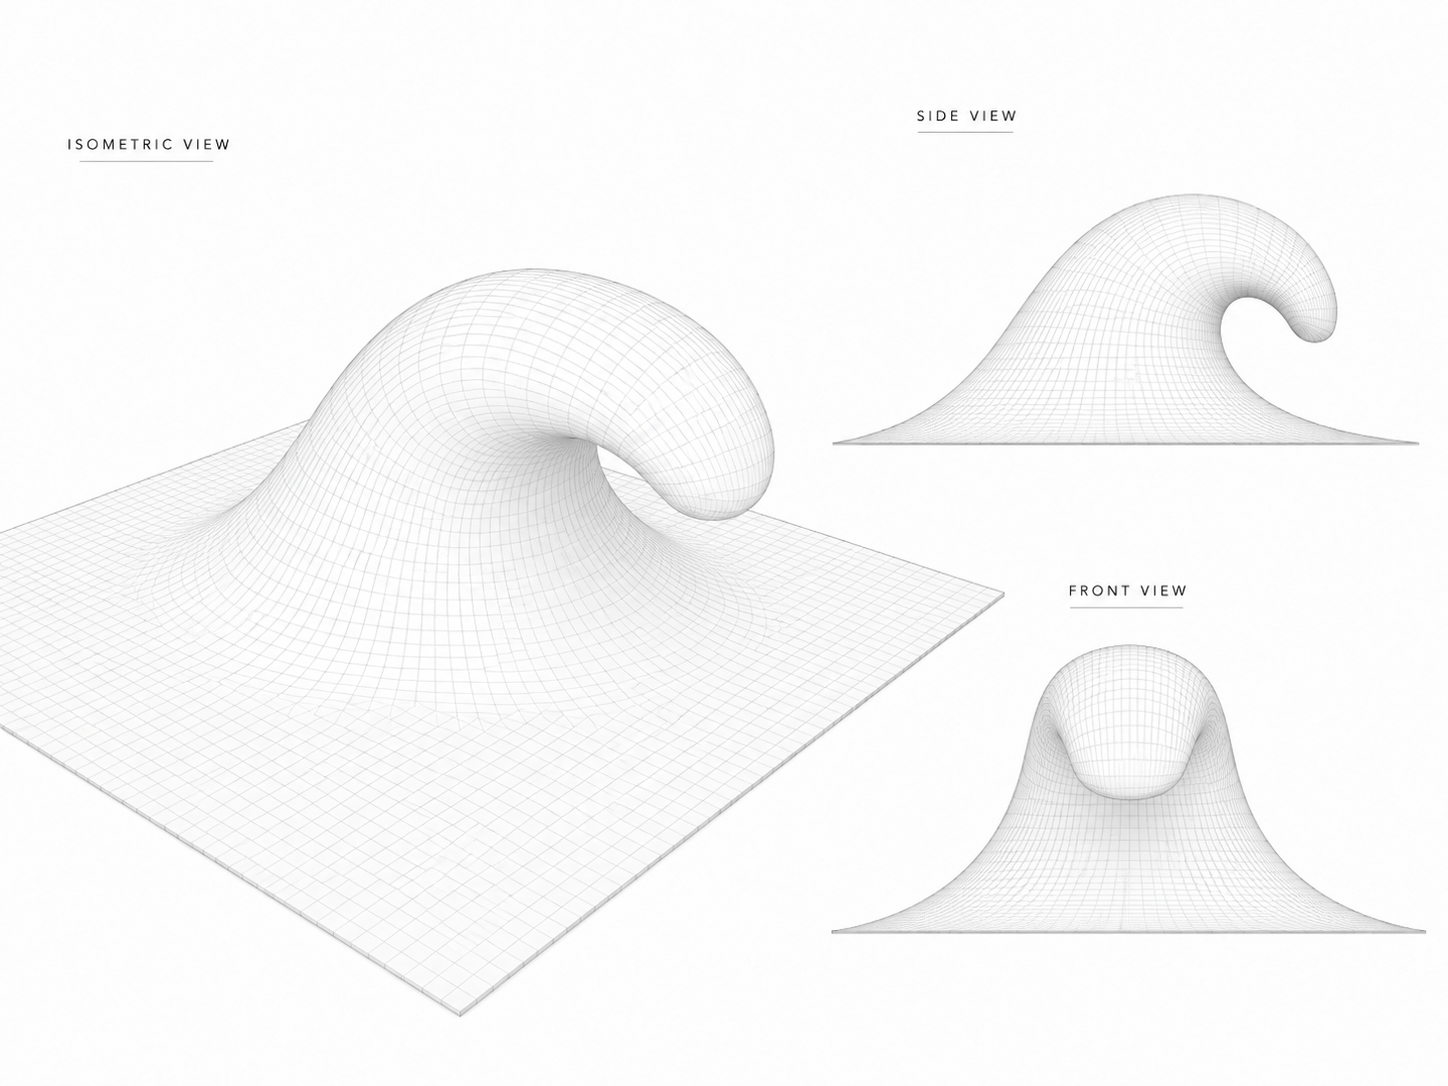
\includegraphics[width=0.98\linewidth]{2026-06-24-smooth-breaking-wave-reference-overview.png}
\caption{June 24 supplied smooth gridded reference overview. Alan re-supplied this image and said ``remember.'' It is now a preserved project reference for the desired visual grammar: a continuous square sheet surface, rounded rising face, tube-like crest, downturned lip, open clean throat, and centered front view. A jagged linkage trace, side-wall tunnel, or metric-only improvement does not satisfy this reference.}
\label{fig:smooth-breaking-wave-reference-overview}
\end{figure}

\begin{figure}[H]
\centering
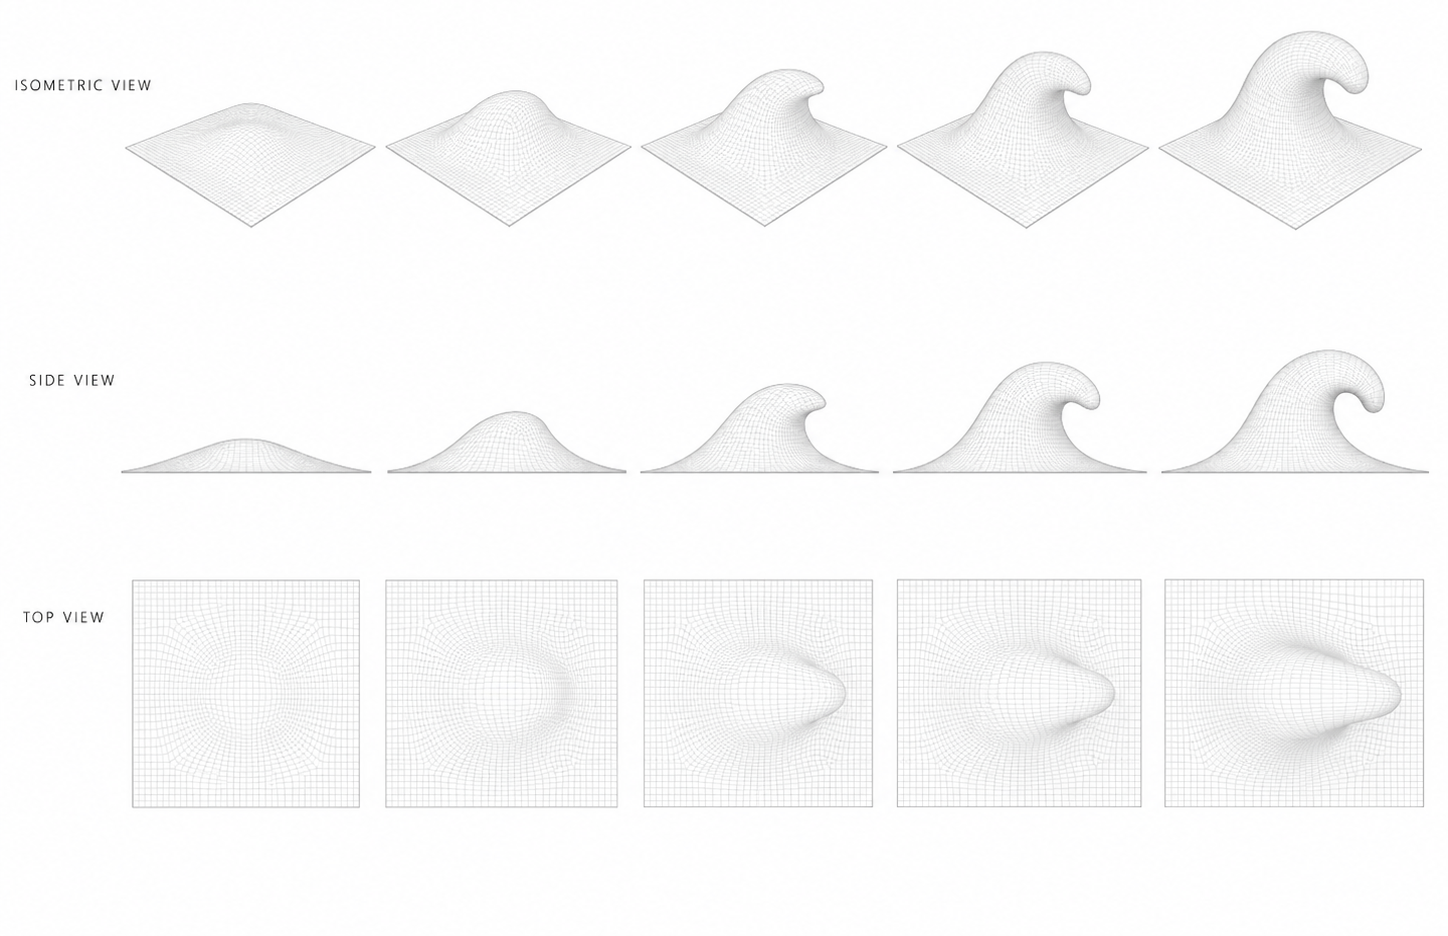
\includegraphics[width=0.98\linewidth]{2026-06-24-smooth-breaking-wave-reference-sequence.png}
\caption{June 24 supplied smooth gridded reference sequence. The sequence records the intended progression across isometric, side, and top views: the deformation grows from a flat square sheet into a localized rounded wave with a curled lip while the top view remains a rounded localized body, not a triangular fan or swept strip.}
\label{fig:smooth-breaking-wave-reference-sequence}
\end{figure}

\begin{figure}[H]
\centering
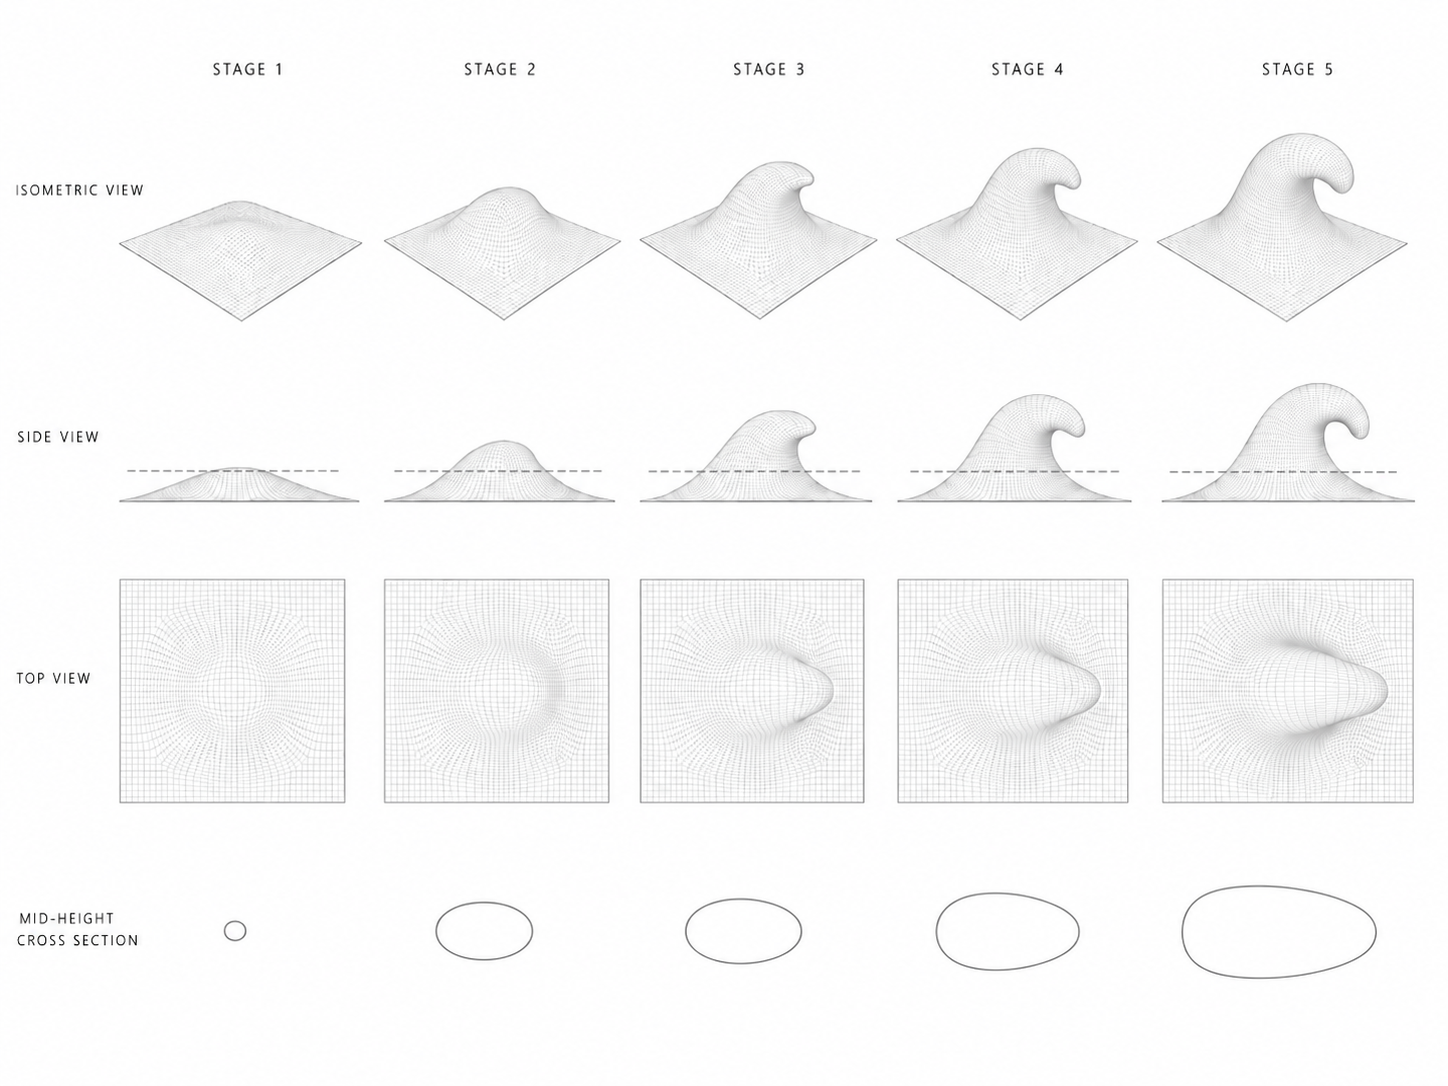
\includegraphics[width=0.98\linewidth]{2026-06-28-wavevis-stage-cross-section-reference.png}
\caption{June 28 supplied stage sequence with an explicit mid-height cross-section row. The bottom row tightens the plan-footprint target: the active body should grow into one smooth oval or teardrop-like section through the curl, not a pointed spear, pinched hourglass, terminal stripe, or pasted helper contour. This reference is now part of the WaveVis acceptance set.}
\label{fig:stage-cross-section-reference}
\end{figure}

\section{Start here for a new WaveVis chat}

If this PDF is the only WaveVis context available, start with this section and then inspect the live artifact. The current project state is:
\begin{itemize}
  \item \textbf{Verified public route:} \code{https://aolabs.io/wavevis/}. This route serves the fallback bundle that Alan actually uses.
  \item \textbf{Working standalone route:} \code{http://wavevis.aolabs.io/}. This route serves the current WaveVis bundle. The HTTPS version remains a separate certificate boundary.
  \item \textbf{Preferred HTTPS route still blocked:} \code{https://wavevis.aolabs.io/}. At the time of this record, HTTPS validation can fail because the custom-domain certificate is not valid for that hostname. Do not treat the HTTPS subdomain as the verified route until a fresh certificate check passes.
  \item \textbf{Visible PDF action:} the WaveVis header links to the paper file under \code{/proofs/}. File: \code{wavevis-system-architecture.pdf}. The old connector proof remains a source artifact, not the primary user-facing paper action.
  \item \textbf{Current source root:} workspace path \code{\_apps/wavevis.aolabs.io/}.
  \item \textbf{Public fallback mirror:} workspace path \code{\_apps/aolabs-site/wavevis/}. A WaveVis deploy to its own \code{gh-pages} branch does not automatically update the \code{aolabs.io/wavevis/} fallback unless the built files are mirrored there and the hub site is pushed.
  \item \textbf{Current architectural direction:} curated supplied-reference field localized into the inverse-sheet model, plus a separate readable display surface for visual inspection. Manual \(xz\) and \(xy\) profile editors are not the active path.
  \item \textbf{Current branch state:} Candidate876 is the last committed baseline source state. It changes \pathcode{src/LatticeViewer3D.tsx} and \pathcode{scripts/check-inverse-sheet.cjs}: segmented side trace, rounded lip-tip control points, slower terminal profile sampler, broadened terminal fold/lift envelopes, sectioned front view, and updated no-point/no-wall/no-terminal-foot gates. It is not accepted as a reference match after the July 1, 2026 pointy-profile complaint. Candidate841 through Candidate875 are rejected or superseded diagnostics that explain support-neck dimples, broad roof/curtain, triangular cut/fin, side-wall tunnel, pointy side profile, full-length front projection, and squared terminal foot failures. Candidate898 through Candidate903 are newer rejected local diagnostics: old smooth trace kept a spiral/pointy side and pinched top; tail release became a blunt cylinder; smooth product profile became a loop/half-pipe; no-loop cap became a mound with no curl; Moana lip anchors made a steep nose without the needed overhang; analytic rounded curl became a broad wall/blob.
  \item \textbf{Current verification state:} \code{scripts/check-geometry-invariants.cjs} passes and \code{npm run build} passes. The local inverse-sheet checker \pathcode{scripts/check-inverse-sheet.cjs} currently fails because the visible mechanism source contract reports \pathcode{sourceUsesConnectedXMechanism=false}. Browser screenshots exist in:
  \begin{quote}\footnotesize
  \pathcode{_verification/}\\
  \pathcode{browser-20260701-}\\
  \pathcode{candidate876-broader-terminal/}
  \end{quote}
  These checks prove that the baseline is buildable and has a runnable mechanism checker; they do not prove that the rendered wave matches the reference family or that the full inverse-sheet gate is closed. The rebuilt PDF, fallback route, and standalone HTTP route were checked on July 1, 2026 for bundle \pathcode{index-SPBHkj_l.js} and the matching public PDF copy, but that checked state is now stale with respect to the latest paper correction until a new PDF/build/deploy cycle is completed. The preferred HTTPS subdomain remains certificate-blocked. The pointy side-profile read, isometric support-cone read, and inverse-sheet visible-mechanism checker failure are still open visual/mechanism debt.
  \item \textbf{Correct acceptance target:} the supplied June 24 smooth breaking-wave reference family and June 28 stage/cross-section reference. The wrong target is any internal trace diagram, centerline overlay, profile-only silhouette, or helper contour that cannot reconstruct the mechanism.
  \item \textbf{Current mechanism contract:} every interior cell is one black square body with four straight legs; opposite leg pairs are equal length and collinear through the cell center; every spherical connector node is a physical two-cell joint with exactly two attached leg uses; crossing diagonal families are separate joints rather than four-cell connector collisions.
  \item \textbf{Do-not-claim boundary:} do not claim reference match, paper current, or public completion from a geometry log, a compiled PDF, a local screenshot, an internal overlay, or a smoother profile string. The rendered full mechanism is the acceptance object.
\end{itemize}

\subsection{What the next agent must not repeat}

The repeated failures that this document is meant to prevent are:
\begin{enumerate}
  \item Do not make a swept tunnel, ribbon, canopy, roof, half-pipe, bridge, or extruded strip.
  \item Do not form a bowl, dimple, cavity, pucker, under-overhang throat bite, or side wall that covers or pinches the underside of the curl.
  \item Do not replace Side with a profile-only debug view. Side is a side camera view of the full three-dimensional sheet.
  \item Do not hide, ghost, clip, or remove linkage cells because they look bad. Fix the geometry.
  \item Do not remove the full array, one-center X cells, exact collinear equal opposite pairs, two-use physical connector joints, or two-cell linkage truth while chasing a prettier outline.
  \item Do not wire the lip directly to the ground or draw filler geometry across the open underside.
  \item Do not make \code{position} or \code{steer} shape controls. They are rigid post-shape transforms.
  \item Do not call the work done from code intent, automated checks, a nicer profile line, or a local-only screenshot.
  \item Do not let the top view collapse into a big triangle, wedge, or V fan while the side view looks acceptable.
  \item Do not paste a mid-height contour, helper ellipse, bridge, or cross-section overlay into the product view to fake the June 28 cross-section row. Fix the surface projection and preserve the X-only proof path.
\end{enumerate}

\subsection{Current state ledger}

This subsection replaces the old Candidate785 figure gallery. Those screenshots are historical diagnostics, not final paper evidence. The paper must not show a stale candidate as if it were the correct geometry. The current ledger is:

\begin{table}[H]
\centering
{\small
\begin{tabular}{@{}Y{0.23\linewidth}Y{0.34\linewidth}Y{0.33\linewidth}@{}}
\toprule
Class & Current source & Paper/display rule \\
\midrule
Accepted references & June 24 smooth gridded overview/sequence, June 28 stage/cross-section reference, and retained ocean-curl photos used only for water-form context. & Keep as target figures and cite them as references, not as achieved WaveVis output. No side-line drawing is accepted as the reference. \\
Rejected display asset & Profile-trace overlay image, black pointy side-profile line, and non-target stills. & Removed from the paper figure sequence; do not use internal trace overlays, side-line surrogates, or visually irrelevant stills as paper figures. \\
Rejected candidate states & Candidate785, Candidate841 through Candidate875, and Candidate898 through Candidate903 screenshots. & Historical diagnostics only. Do not describe them as accepted renders after Alan identified support-neck, pointy-profile, front-fin, wall, blob, cone, terminal-foot, blunt-cylinder, half-pipe, no-curl mound, steep-nose, and broad-wall families. \\
Current source baseline & Candidate876 viewer and checker changes: segmented side trace, rounded lip-tip anchors, terminal sampler slowdown \(0.064\), broadened terminal fold/lift envelopes, sectioned front view from the shared 3D reference field, no-point/no-wall/no-terminal-foot gates, flat perimeter, and visible mechanism locks. & Useful as a committed baseline and source of invariant checks only. The visual reference match remains open because the current side profile and isometric support-cone read do not match the accepted gridded reference family. \\
Mechanism invariant & One-center four-leg X cells with exact opposite-pair collinearity/equal length and physical two-use connector nodes. & Keep as a hard gate and cite source/checker values after each accepted candidate. \\
Open boundary & Correct rounded reference-family match, public/fallback route parity, and PDF figure/source consistency. & Blocks final paper claims, deployment claims, and Progress closure until live routes and PDF renders are verified. \\
\bottomrule
\end{tabular}
}
\caption{WaveVis state ledger as of July 1, 2026. The paper tracks which information is reference truth, rejected history, active source state, and still-open defect state.}
\label{tab:current-ledger}
\end{table}

The only current figures that belong in the paper by default are target references and mechanism-proof figures that still define the actual constraint. Candidate screenshots belong only when they are labeled as rejected or diagnostic and they help the next iteration avoid a known failure.

\subsection{Figure and asset hygiene}

WaveVis now treats paper figures as source evidence, not decoration. A file can appear in this PDF only if it belongs to one of four classes:
\begin{enumerate}
  \item a target reference that defines the accepted geometry family;
  \item a current accepted render that passed source checks, browser inspection, and route verification;
  \item a mechanism proof figure that defines a hard constraint still used by the source;
  \item a clearly labeled rejected diagnostic that explains a failure mode future iterations must avoid.
\end{enumerate}
Profile-trace overlays, centerline-only comparisons, stale candidate screenshots, unrelated stills, helper contours, and any image whose purpose is to make the current source look more correct than the rendered mechanism must stay out of the paper and the public proof folder. When an asset is removed for this reason, the removal is part of the source-of-truth record rather than cleanup churn.

\subsection{File map}

\begin{table}[H]
\centering
{\footnotesize
\begin{tabular}{Y{0.43\linewidth}Y{0.48\linewidth}}
\toprule
File or route & Ownership \\
\midrule
\code{src/latticeGeometry.ts} & Source of truth for the inverse sheet model, defaults, sanitization, target displacement field, morph behavior, metrics, and geometry sanity checks. \\
\code{src/LatticeViewer3D.tsx} & Source of truth for Canvas rendering, side/isometric/top full-sheet camera behavior, surface visibility, camera presets, visual layers, and the rendered collinear equal-pair X-cell and shared-joint layers. \\
\code{src/xCellMechanism.ts} & Source of truth for the connected X-cell display mechanism: one black-square cell body per lattice cell, four straight center-to-connector legs per cell, exact collinear/equal opposite pairs through the cell center, and spherical connector nodes with exactly two attached leg uses. \\
\code{src/TargetShapeControls.tsx} & Source of truth for the visible inverse-sheet controls: rows, columns, views, scale, morph, position, steer, display toggles, reset, export, and import. \\
\code{src/InverseSheetTab.tsx} & Source of truth for URL-state loading, tab order, view requests, import/export plumbing, and the Inverse Sheet first-tab behavior. \\
\code{scripts/check-inverse-sheet.cjs} & Main inverse-sheet regression checker. It compiles the TypeScript geometry and checks parameter semantics, lip curl, flatContribution, low-lip stability, lateral smoothness, no bowl pockets, terminal taper, startup URL coverage, and the collinear equal-pair X-cell render contract. \\
\code{scripts/check-geometry-invariants.cjs} & Mechanism-level invariant checker for rigid-cell/linkage behavior. \\
\code{proofs/wavevis-system-architecture.tex} & Source for this PDF. Update it when the public simulator contract, current state, or known failure modes change. \\
\code{proofs/figures/} & Project-defining reference images and mechanism proof figures used by this paper. Old current-state screenshots and trace overlays must stay out of the paper unless explicitly labeled as rejected diagnostics. \\
\code{dist/} & Built WaveVis static app after \code{npm run build}. Do not edit by hand. \\
\code{aolabs-site/wavevis/} & Public fallback mirror for \code{https://aolabs.io/wavevis/}. Copy the built \code{dist} contents here when the public fallback must update. \\
\bottomrule
\end{tabular}
}
\caption{Current source map. A new WaveVis chat should use these files rather than reconstructing behavior from old prompts.}
\end{table}

\subsection{Minimal continuation workflow}

A fresh agent continuing WaveVis should do the following in order:
\begin{enumerate}
  \item Read this PDF and \code{src/latticeGeometry.ts}, then inspect \code{src/LatticeViewer3D.tsx} and \code{src/TargetShapeControls.tsx}.
  \item Open the verified public route \code{https://aolabs.io/wavevis/} and the current local route if a dev server is running.
  \item Reproduce Alan's active preset from the URL before changing source. Do not judge a different default state.
  \item Run \code{npm run check:geometry}. If it fails, fix source before visual tuning.
  \item Render and inspect \code{Side}, \code{3D}, and \code{Top}. Side and 3D must both be full-sheet views with the curl visible.
  \item Make the smallest source change that improves the human-facing breaking-wave outcome without regressing the mechanism invariants.
  \item Re-run \code{npm run check:geometry} and \code{npm run build}.
  \item Verify live/public output after deploy or fallback mirror update. A local screenshot is not the public artifact.
  \item Update this PDF if the architecture, current state, source map, controls, or known failure classes changed.
  \item Post a Progress event with complaint, issue, Codex change, observed source change, provenance, and commit ids.
\end{enumerate}

\section{Current implementation state}

\subsection{Defaults and target}

The current inverse-sheet default is intentionally taller and sharper than earlier flat presets:
\[
\begin{aligned}
\code{rows}&=44,&
\code{columns}&=112,&
\code{morph}&=1,\\
\code{height}&=15.25,&
\code{horizontalOffset}&=22.5,&
\code{overhangWidth}&=32,\\
\code{overhangAngleDeg}&=120,&
\code{overhangPosition}&=-0.15,&
\code{profileScale}&=0.60,\\
\code{smoothing}&=1,&
\code{lipSharpness}&=0.50,&
\code{wallSmoothness}&=0.28,\\
\code{flatContribution}&=0.35.
\end{aligned}
\]
The app displays only the narrow active controls by default. Legacy inputs such as \code{height}, \code{overhang}, \code{lipDip}, \code{width}, \code{lipSharpness}, \code{groundTransition}, \code{wallSmoothness}, and \code{flatContribution} can still be parsed from URLs and JSON imports because older test links and screenshots use them. The visible startup path favors \code{scale}, \code{morph}, \code{position}, and \code{steer} to keep the main wave profile stable.

The default reference-wave sheet remains \(\code{columns}=112\). The sanitizer now allows \(\code{columns}\ge 12\) so X-cell proof routes can be inspected at low density, but compact column counts are not evidence of an exact reference-wave match. Dense-wave regression checks request the default column count explicitly; low-column screenshots are mechanism-readability proofs.

\subsection{Target-field construction}

The target is constructed in a canonical wave frame. The canonical frame removes \code{position} and \code{steer}; the shape is computed there; then steer and position are applied as rigid transforms afterward. This prevents the old bug where moving the wave also changed its profile.

The source sequence in \code{buildNodes} is:
\begin{enumerate}
  \item build rest grid \(p^0_{ij}\);
  \item compute core target positions from \code{targetFromDeformationField};
  \item pin perimeter nodes to rest;
  \item apply span continuity smoothing for generated mode;
  \item apply flat-contribution diffusion as a support apron, not as a flattening blend;
  \item interpolate from rest to target with \code{morphGrowthAmount};
  \item build metrics, edges, quads, and dihedral pairs from the resulting grid.
\end{enumerate}

The target function samples \(u\) along the wave field and \(v\) across span:
\[
  u = \frac{x-x_{\min}}{L}, \qquad
  v = \frac{y + S/2}{S}.
\]
The displacement is zero outside the support field and on the perimeter. The support field expands with \code{smoothing} and \code{flatContribution}, but the core wave must remain the same shape.

\subsection{Reconstruction-grade mathematical model}

Let the rest sheet be a rectangular lattice with \(R\) rows and \(C\) columns. In source, \(R=44\), \(C=112\), rest sheet length \(L_s=80\), rest sheet span \(S_s=80\), wave-field length \(L=43\), and wave-field span \(S=43\). A node is
\[
  p^0_{ij} =
  \begin{bmatrix}
    -L_s/2 + jL_s/(C-1)\\
    -S_s/2 + iS_s/(R-1)\\
    0
  \end{bmatrix},
  \qquad
  0\le i<R,\quad 0\le j<C.
\]
Boundary nodes are hard pinned:
\[
  p^*_{ij}=p^0_{ij}\quad\text{if}\quad i\in\{0,R-1\}\ \text{or}\ j\in\{0,C-1\}.
\]
For interior nodes, WaveVis maps the world point into a canonical wave frame by removing user placement:
\[
\begin{aligned}
  \tilde p &= R_z(-\psi)\left(p^0 - a - \delta_x e_x\right)+a,\\
  \psi &= \frac{\pi}{4}\clamp(\code{steer},-1,1),\\
  \delta_x &= 0.045L\clamp(\code{position},-1,1).
\end{aligned}
\]
The canonical target is
\[
  \tilde p^* = \tilde p + D(\tilde x,\tilde y;\theta),
\]
and the world target is restored by applying the inverse rigid placement. This separation is required because inverse-design controls should not silently change the target surface. It follows the same general separation used in graphics simulators between state variables, constraints, and display transforms~\cite{muller_position_based_2007,bouaziz_projective_2014}.

The active source contains two target/display paths that must not be confused:
\begin{enumerate}
  \item \textbf{Model target path,} owned by \code{src/latticeGeometry.ts}. It generates node targets, metrics, and the mechanism-check state.
  \item \textbf{Readable display path,} owned by \code{src/LatticeViewer3D.tsx}. It draws a reference-like gridded surface and mechanism layer for visual inspection. It is not allowed to replace the model target or hide invalid mechanism state.
\end{enumerate}

\subsubsection{Custom profile path}

When \code{profileMode='custom'}, the model source uses serialized control points. The last committed Candidate876 baseline centerline source is:
\[
\begin{split}
&(0,0),(0.04,0.008),(0.095,0.033),(0.17,0.105),(0.275,0.305),\\
&(0.385,0.58),(0.5,0.82),(0.61,0.965),(0.69,1),(0.78,0.965),\\
&(0.858,0.86),(0.922,0.704),(0.967,0.528),(0.985,0.384),\\
&(0.965,0.3),(0.937,0.228),(0.919,0.16),(0.934,0.092),\\
&(0.971,0.037),(1,0).
\end{split}
\]
Those are normalized \((x,z)\) anchors, not final mechanism coordinates and not an accepted visual reference. They are sampled, scaled, localized across the span, morph-interpolated, and then checked against the mechanism constraints. After the July 1, 2026 pointy-profile complaint, this point list should be treated as a baseline to replace or repair, because the rendered side read is still too pointy for the accepted gridded reference family. If a future candidate changes this profile, it must record the new point list, the reason for every moved anchor, and the rendered visual failure it fixes.

\subsubsection{Generated lip path}

The generated path uses a ramp/crest/lip decomposition:
\[
  P(u)=
  \begin{cases}
    P_{\mathrm{ramp}}(u), & 0\le u<u_c,\\
    P_{\mathrm{crest}}(u), & u_c\le u<u_l,\\
    P_{\mathrm{lip}}(u), & u_l\le u\le1.
  \end{cases}
\]
In source, \code{moanaReferenceLipPoints} builds a normalized list of lip anchors controlled by \code{dip} and \code{sharp}. The anchors are smoothed into cubic Bezier segments, then sampled by normalized arc length:
\[
  q(\alpha)=B_k(t)\quad\text{where}\quad
  \sum_{\ell<k}\int_0^1\norm{B'_\ell(s)}\,\dd s+
  \int_0^t\norm{B'_k(s)}\,\dd s
  =\alpha\,\ell_{\mathrm{total}}.
\]
The source samples this curve numerically using 18 subdivisions per cubic segment. A future exact reconstruction should replace that sampling with an analytic or higher-resolution arc-length inversion only if the rendered mechanism improves and the validation gates still pass.

\subsubsection{Span localization}

The readable display path uses a lateral envelope
\[
  E(s)=\cos^{1.42}\left(\frac{\pi}{2}|s|\right), \qquad s\in[-1,1],
\]
then uses powers of \(E\) near the terminal lip to localize the curl. The source intentionally makes the lip narrower than the broad ramp; otherwise a centerline curl becomes a swept tunnel. Candidate876 kept the terminal localization bounded and lowered the powers from the old center-spike setting, but the rendered result is now only a baseline because the side profile remains too pointy and the isometric support-cone read remains visible:
\[
  \tau(t)=\operatorname{clamp}_{[0,1]}\left(t-0.064\sin\left[\pi S(0.68,1,t)\right]\right),
\]
\[
  F_{\mathrm{fold}}(s,t)=\operatorname{lerp}\left(F_{\mathrm{shoulder}},E(s)^{1.78},0.58\,S(0.70,1,t)\right),
\]
\[
  F_{\mathrm{lip}}(s,t)=\operatorname{lerp}\left(E(s)^{1.18},E(s)^{1.90},0.68\,S(0.70,1,t)\right).
\]
The sampler \(\tau(t)\) was intended to keep the lower curl inside the rounded hook before releasing to the flat tail. It does not currently prove a correct side profile. Candidate876 also keeps the crest-cap exception around the rounded lip:
\[
  C(t)=S(0.54,0.66,t)\,[1-S(0.82,0.94,t)],
\]
\[
  H_{\mathrm{cap}}(s)=\left(1-S(0.20,0.82,|s|)\right)^{0.78},
\]
and blends the height span toward \(H_{\mathrm{cap}}\) with weight \(0.86C(t)\). This is not a tunnel relaxation. It is the blocker against the opposite failure Alan identified: a pointy fin or spike in the front/cross-section view. In the model path, the same localization principle appears through \code{transverseSupportMask}, \code{lipAwareRimMask}, \code{terminalLipSpanMask}, \code{shapeMask}, and the post-core taper terms.

\subsubsection{Bowl/dimple blocker}

The source blocker \code{blockSurfaceBowlPockets} runs before node emission. For each interior node with active neighboring height, it replaces a local low point by the minimum of its four direct neighbors:
\[
  z_{ij}^{(k+1)} =
  \max\left(z_{ij}^{(k)},\min(z_{i-1,j}^{(k)},z_{i+1,j}^{(k)},z_{i,j-1}^{(k)},z_{i,j+1}^{(k)})\right),
\]
for up to six passes. This is a pre-render invariant sweep, not a visual cleanup. It catches bowl-like local minima, but it is not sufficient for the under-overhang support-neck failure; that failure also requires side/isometric throat sampling and human-facing render inspection.

\subsubsection{Connected X-cell equations}

For each node center \(c_n\), the visible cell is one square body with four legs in directions \(\{\mathrm{NE},\mathrm{SW},\mathrm{NW},\mathrm{SE}\}\). For each opposite pair,
\[
  \norm{e_{\mathrm{NE}}-c_n}=\norm{e_{\mathrm{SW}}-c_n}, \qquad
  e_{\mathrm{NE}}+e_{\mathrm{SW}}=2c_n,
\]
and similarly for \(\mathrm{NW}/\mathrm{SE}\). The same connector point \(g_{ab}\) is shared by exactly two adjacent cells:
\[
  e_{a,+}=g_{ab}=e_{b,-}, \qquad \#\{(n,d): e_{n,d}=g_{ab}\}=2.
\]
The current source solves connector chains by alternating signs along each row/column family:
\[
  g_0=f,\qquad
  g_k=2c_k-g_{k-1}\quad(k>0),
\]
then chooses \(f\) by least-squares midpoint residual over the adjacent pair family. This preserves exact cell-level opposite-pair closure and exposes center-corridor drift as a diagnostic rather than hiding it. The checker then groups connector positions by physical coordinate, not only by id, so two connector ids occupying one point cannot create a silent four-cell joint.

\subsubsection{Acceptance objective}

WaveVis is not currently optimizing a single scalar objective. The useful mental model is a constrained inverse-design problem:
\[
  \min_{\theta,\mathcal{G}}\ 
  w_r E_{\mathrm{ref}}(\Phi_\theta,\Phi_{\mathrm{ref}})
  +w_s E_{\mathrm{smooth}}
  +w_m E_{\mathrm{mechanism}}
  +w_v E_{\mathrm{view}}
\]
subject to boundary pinning, topology completeness, connector occupancy, no bowl/dimple pockets, and public route verification. At this stage the objective is enforced as explicit gates rather than a continuous solver: reference match is judged on the rendered object; mechanism feasibility is checked in source; stale paper/public assets are treated as failures.

For a future continuous solver, the scalar terms should be reconstructed from the current gates rather than invented from scratch. A practical decomposition is:
\[
\begin{aligned}
E_{\mathrm{ref}} &= \lambda_s D_{\mathrm{side}}\!\left(S_{\mathrm{side}},R_{\mathrm{side}}\right)
  + \lambda_t D_{\mathrm{top}}\!\left(S_{\mathrm{top}},R_{\mathrm{top}}\right)
  + \lambda_f D_{\mathrm{front}}\!\left(S_{\mathrm{front}},R_{\mathrm{front}}\right)
  + \lambda_o\,E_{\mathrm{open}},\\
E_{\mathrm{smooth}} &= \sum_{(i,j)} \norm{\Delta^2_x p_{ij}}^2+\norm{\Delta^2_y p_{ij}}^2,\\
E_{\mathrm{mechanism}} &= \sum_n\left(
  \epsilon_{\mathrm{oppLen}}(n)^2+
  \epsilon_{\mathrm{oppCol}}(n)^2+
  \epsilon_{\mathrm{jointUse}}(n)^2+
  \epsilon_{\mathrm{anchor}}(n)^2
\right),\\
E_{\mathrm{view}} &= \epsilon_{\mathrm{sideWall}}^2+\epsilon_{\mathrm{skinnySail}}^2+\epsilon_{\mathrm{frontPoint}}^2+\epsilon_{\mathrm{frontWall}}^2+\epsilon_{\mathrm{pointyProfile}}^2+\epsilon_{\mathrm{hiddenMech}}^2.
\end{aligned}
\]
Here \(R_{\mathrm{side}},R_{\mathrm{top}},R_{\mathrm{front}}\) are view-level targets extracted from the accepted gridded reference family, not from the rejected black line drawing. \(D_{\mathrm{side}}\) may include a Fréchet-like curve-distance term after a side contour is extracted from the full sheet, but that term is invalid if the top, front, open-throat, or mechanism-visibility terms fail. \(E_{\mathrm{open}}\) samples the underside throat below the lip for dimples, bites, bowls, and support-necks, and \(D_{\mathrm{top}}\) rejects broad terminal blobs, triangles, and V fans in plan view. \(E_{\mathrm{frontPoint}}\) rejects a rounded-wave front view that collapses into a vertical fin; \(E_{\mathrm{frontWall}}\) rejects the opposite full-width wall; \(\epsilon_{\mathrm{pointyProfile}}\) rejects a sharp or needle-like side silhouette even when the outer curl radius appears continuous. This follows the general inverse-design pattern of optimizing a physically meaningful state subject to explicit manufacturability and simulation constraints~\cite{skouras_designing_inflatable_2014,konakovic_auxetic_2016,panetta_surface_inflatables_2021,du_diffpd_2022}, but WaveVis should keep the gate form until the rendered artifact is stable enough that a scalar objective would not hide a visible failure.

\subsubsection{Candidate iteration record}

Every new geometry candidate must be traceable. The minimum record is:
\[
  \mathcal{R}_k=
  \{\text{candidate id},\text{source diff},\text{intended defect},\text{metrics},\text{render captures},\text{accept/reject reason}\}.
\]
The accept/reject reason must name the rendered shape, not only the code change. A valid note says, for example, ``rejected: side open throat improved but top became a broad terminal blob.'' An invalid note says only ``geometry check passed.'' Candidate848 through Candidate875 are examples of why this record matters: some local gates passed, but browser renders still showed support ridges, broad top blobs, front-wall reads, pointy fin profiles, squared terminal feet, or support-cone reads. Candidate876 is the current committed baseline only; its build pass and geometry-invariant pass do not override the rendered pointy-profile defect, support-cone defect, or the current inverse-sheet visible-mechanism checker failure. Candidates 898 through 903 extend the rejection ledger: old smooth trace kept a spiral/pointy side and pinched top; tail release became a blunt cylinder; smooth product profile became a loop/half-pipe; no-loop cap became a mound with no curl; Moana lip anchors made a steep nose without the needed overhang; analytic rounded curl became a broad wall/blob.

\subsection{Rigid controls}

\code{position} and \code{steer} are post-shape placement controls:
\[
  \Delta x_{\mathrm{position}} = 0.045\,L\,\mathrm{clamp}(\code{position},-1,1),
\]
\[
  \psi_{\mathrm{steer}} = 45^\circ\,\mathrm{clamp}(\code{steer},-1,1).
\]
They must not modify the curated wave profile, width, curl, strain, or topology. Validation aligns geometries back to the canonical frame and checks that residual shape differences are near zero for position and bounded for steer.

\subsection{Morph control}

\code{morph} is not a shape recipe. It interpolates from rest to the completed target:
\[
  p_{ij}(m) = (1-g(m))p^0_{ij} + g(m)p^*_{ij}.
\]
The current growth function combines a sine ease with a faster visible growth curve so the wave grows naturally without a dead early range. Morph must preserve topology, connector closure, and the visible wave identity throughout the range. If \(\code{morph}=0.5\) produces zig-zags, overlaps, missing cells, or a side-wall-covered curl, that is a geometry failure.

\subsection{Flat contribution and ground transition}

\code{flatContribution} does not mean flatten the wave. It means share deformation with the surrounding sheet through a support apron. In accepted behavior:
\begin{itemize}
  \item the main wave height and overhang reach stay within a small residual;
  \item the centerline profile remains essentially unchanged;
  \item surrounding flat areas participate more gradually;
  \item strain concentration is reduced or spread rather than hidden.
\end{itemize}
The old behavior \(\code{target}=\mathrm{lerp}(\code{deformed},\code{rest},\code{flatContribution})\) is explicitly rejected because it turns \code{flatContribution} into a flattening slider.

\code{smoothing}, shown historically as ground transition, broadens the support field and root ramp. It should recruit surrounding flat sheet into the slope while keeping the perimeter pinned and preserving the terminal lip.

\subsection{Lip dip and terminal curl}

\code{lipDip} maps to \code{overhangAngleDeg}. Neutral is \(90^\circ\). High curl is \(120^\circ\). The accepted behavior is not endpoint lowering. The wave should rise, crest, reach forward, curl downward, then return smoothly to the flat sheet without closing into a bowl. The current validation checks:
\begin{itemize}
  \item the selected lip nose is a mid-height visible point below the last peak, not the near-floor return;
  \item the terminal slope is negative;
  \item the tip is forward of the crest and tucked under the shoulder by a bounded amount;
  \item the return advances toward the flat front instead of folding backward;
  \item the terminal cavity blocker, backfold blocker, and visible-dimple blocker remain true.
\end{itemize}
These checks are guards, not substitutes for the human-facing screenshot. A visible dimple, under-overhang pocket, side wall, or missing curl still means open work.

\subsection{Rendering contract}

\code{LatticeViewer3D.tsx} renders the readable surface and a connected X-cell mechanism from the actual lattice graph. In the current contract:
\begin{itemize}
  \item \code{view=side} sets a side camera over the full three-dimensional linkage array;
  \item \code{view=front} sets a front camera over a crest-section window sampled from the same readable three-dimensional field, so the view inspects the rounded cross-section instead of projecting the whole side trace into a fin;
  \item \code{view=isometric} shows the full rectangular sheet in perspective while still making the curl and lip readable;
  \item the default product view uses a smooth gridded surface skin plus one-center four-leg X-cell leg lines, black square cell bodies, and spherical connector nodes;
  \item Side, Front, and 3D use view-specific mesh outlines instead of the previous SVG overlay, centerline comparison, or red terminal trace;
  \item each rendered X cell is one black square cell body with four visible center-to-connector legs;
  \item each connector is a spherical two-use physical node between adjacent cells;
  \item each connector has exactly two endpoint uses: one leg from each of those two centers;
  \item crossing diagonal families must stay visually and physically separate instead of collapsing into a four-cell joint;
  \item connector corridor drift is reported as a bounded diagnostic when exact cell-level opposite-pair closure moves a connector away from the old midpoint corridor;
  \item cells and X legs are display toggles, not repair paths, and their render scope remains covered by the geometry check.
\end{itemize}
If the renderer needs to hide rows to make the shape readable, the generator is still wrong.

\section{Target outcome}

\subsection{Human-facing shape}

The accepted target is a ``flat sheet plus localized plunging wave'':
\begin{itemize}
  \item the outer perimeter of the rectangular sheet remains flat and fixed;
  \item the wave emerges through a broad, smooth ramp rather than a vertical wall;
  \item the crest is rounded, with no top dent;
  \item the lip projects forward and curls downward;
  \item the open underside is visible from side view, not covered by a side wall;
  \item the shape fades back to flat in every direction;
  \item the array remains a full linkage field with nodes and legs, not a hidden or clipped shell.
\end{itemize}

The practical acceptance boundary is a projected full-sheet condition, not a standalone drawn profile. Let the rest sheet be \(\Omega=[-1,1]\times[-1,1]\) with boundary \(\partial\Omega\), sampled by linkage nodes \(r_{ij}=(x_i,y_j,0)\), and let the generated mechanism state be \(p_{ij}=\Phi_\theta(r_{ij})\). A future candidate is eligible for visual review only if
\[
  \max_{r_{ij}\in\partial\Omega}\norm{p_{ij}-r_{ij}}\le\varepsilon_{\partial},
  \qquad
  \mathcal{V}_{\mathrm{mech}}(p,\mathcal{G})=1,
\]
where \(\mathcal{V}_{\mathrm{mech}}\) means full visible cell bodies, four straight legs per cell, two-use connector joints, and no hidden filler geometry. The side, top, front, and isometric views are then projections of the same state:
\[
  S_{\mathrm{side}}=\Pi_{xz}\{p_{ij}\},\quad
  S_{\mathrm{top}}=\Pi_{xy}\{p_{ij}\},\quad
  S_{\mathrm{front}}=\Pi_{yz}\{p_{ij}\}.
\]
The candidate must satisfy all three projected readings at once: broad rounded side curl, rounded localized top footprint, and rounded front/cross-section body. A side-line surrogate is rejected even if it looks clean in isolation, because it cannot encode span localization, open throat clearance, perimeter flatness, or mechanism visibility.

\subsection{Hard constraints}

The WaveVis generator and renderer must preserve the following hard constraints:
\begin{enumerate}
  \item \textbf{Flat perimeter.} Boundary nodes must remain on the rest sheet. No side, front, or rear perimeter should be pulled into the wave.
  \item \textbf{Full array visibility.} The rendered artifact must show the actual linkage grid. Hiding or ghosting broken cells does not count as a fix.
  \item \textbf{Connector closure.} A cell connector is an actual shared graph location. Lines should meet at nodes; apparent detached legs are a failure.
  \item \textbf{No erratic legs.} Long arms, spikes, zig-zags, random backtracking, and visible overlaps indicate a broken geometry or render path.
  \item \textbf{Smooth strain sharing.} Adjacent rows and columns should change gradually enough that the mesh reads as a continuous mechanism field.
  \item \textbf{Localized wave.} The curl must be strongest near the center and fade laterally. A constant side-to-side tunnel is not the target.
  \item \textbf{Full-view side semantics.} Side view shows the full three-dimensional render from the side. It must not be replaced by a profile-only debug view.
  \item \textbf{No filler geometry.} Cosmetic walls, caps, planks, bridges, hidden couplers, or masks must not be used to conceal a bad mechanism.
\end{enumerate}

\section{Coordinate model}

The simulator starts from a rectangular rest lattice. A node with row \(i\) and column \(j\) has rest position
\[
  p_{ij}^{0} = (x_j, y_i, 0).
\]
The target is a displacement field
\[
  p_{ij}^{*} = p_{ij}^{0} + m\,D(x_j,y_i;\theta),
\]
where \(m\in[0,1]\) is the morph amount and \(\theta\) represents all shape parameters except rigid placement. The morph parameter only interpolates between rest and the finalized target. It must not change the target shape definition, remesh the lattice, or introduce a different topology.

The longitudinal coordinate \(u\in[0,1]\) measures progress through the wave region from rear/root to front/lip. The span coordinate \(v\in[-1,1]\) measures lateral distance from the centerline. A good WaveVis target uses both:
\[
  D(x,y) = A(u,v)\,P(u) + B(u,v)\,Q(u),
\]
where \(P(u)\) is the side-profile contribution, \(Q(u)\) can include forward curl or secondary displacement terms, and \(A,B\) are smooth two-dimensional envelopes that go to zero at the sheet perimeter.

The key architectural rule is that \(A(u,v)\) is not constant in \(v\). A constant span envelope turns any attractive profile into a tunnel. A localized plunging wave requires \(A(u,0)\) large near the centerline and \(A(u,\pm1)\approx0\) near the sides, with a monotone or smoothly unimodal falloff rather than a hard wall.

\section{Generation pipeline}

The target-building pipeline is:
\begin{enumerate}
  \item sanitize rows, columns, visible sliders, hidden legacy shape parameters, display flags, and URL parameters;
  \item build the full rectangular node grid;
  \item compute the canonical rounded breaking-wave displacement from the supplied reference target;
  \item apply the span envelope that localizes the wave in \(y\);
  \item preserve the boundary by forcing perimeter displacement to zero;
  \item apply morph interpolation from rest to target;
  \item apply rigid steer and position transforms after the shape is finalized;
  \item build full rectangular edge and quad topology;
  \item compute strain, bend, shear, dihedral, and display metrics;
  \item render the full array, side view, 3D view, and top view without substituting fake surfaces.
\end{enumerate}

The distinction between the supplied reference target and rigid placement parameters is essential. The visible app no longer exposes manual \(xz\) or \(xy\) profile editors. The source target owns the rounded breaking-wave profile. The user-facing sliders are intentionally narrow: scale uniformly resizes that target, morph blends from rest to the completed target, steer rotates the finished target around the anchor, and position translates the finished target horizontally. Neither steer nor position may feed back into profile curvature, curl, width, strain generation, or cell topology.

\begin{table}[H]
\centering
{\small
\begin{tabular}{@{}Y{0.22\linewidth}Y{0.37\linewidth}Y{0.30\linewidth}@{}}
\toprule
Stage & Contract & Failure caught \\
\midrule
Target profile & Defines the desired side profile shape. & Blob, neck/head, hill without lip, top dent. \\
Span envelope & Localizes the wave in the sheet. & Swept barrel, side wall, U-shaped tube blocker. \\
Boundary clamp & Keeps the perimeter flat. & Pulled sheet edges, non-flat perimeter. \\
Morph & Interpolates rest to target only. & Half-morph mangling, topology change while sliding. \\
Topology & Keeps full node/edge/quad graph. & Missing grid, hidden cells, detached legs. \\
Renderer & Shows the actual mechanism. & Fake shell, hidden wall, side view as profile-only debug output. \\
Paper evidence & Includes only target references, accepted mechanism proofs, accepted current renders, or clearly labeled rejected diagnostics. & Stale candidate screenshots, misleading overlays, and internal trace diagrams appearing as authoritative figures. \\
\bottomrule
\end{tabular}
}
\caption{Pipeline stages and the failure modes each stage must prevent.}
\end{table}

\section{Supplied rounded target}

The current visible app does not ask the user to draw a profile. That path created too much ambiguity and repeatedly made the simulator look like a swept tunnel or hand-edited cavity rather than a single coherent wave. The user-facing target is now driven by the supplied rounded breaking-wave lip/body profile: a localized ocean deformation with a broad rear ramp, rounded crest, forward-and-down lip, open underside, smooth lateral fade, and flat rectangular perimeter.

The curated target is a reference field, not a set of cell locations. The final cell grid is determined by row and column counts, then sampled against that target. A clean state must keep the full linkage array visible while making the centerline and lateral profile read as one plunging wave. The target must never stitch the lip directly to the ground or draw a hard polygon boundary around a former editor curve, because that creates the wall, bowl, cavity, and silhouette-only failures this record explicitly rejects. The curl is also resolution-sensitive: the default reference-wave state keeps \(112\) columns, while reduced column counts are reserved for low-density mechanism inspection and must not be mistaken for a completed reference-shape view.

\section{Slider semantics}

\begin{table}[H]
\centering
{\small
\begin{tabular}{@{}Y{0.24\linewidth}Y{0.32\linewidth}Y{0.33\linewidth}@{}}
\toprule
Control & Intended effect & Must not do \\
\midrule
\code{morph} & Blend rest sheet into the completed target. & Remesh, flip cells, create zig-zags, change profile identity. \\
\code{scale} & Uniformly enlarge or reduce the supplied rounded target. & Change steer, position, topology, or the target's wave identity. \\
\code{steer} & Rigid yaw rotation of the finished wave. & Bend, stretch, or reshape the wave. \\
\code{position} & Rigid horizontal translation of the finished wave. & Change profile, strain field, or curl. \\
display toggles & Surface, flat grid, cells, and X legs are display layers only. & Hide broken geometry or substitute a fake repair path. \\
\bottomrule
\end{tabular}
}
\caption{Visible control contract after removing manual profile editors and hidden shape sliders. The supplied rounded target is the default shape; visible controls must preserve that shape unless their narrow role explicitly changes scale, morph, steer, position, or display layers.}
\end{table}

\section{Breaking-wave geometry}

The desired default profile is closer to a localized plunging wave than to a cone, cylinder, or arch. The useful approximation is a tapered, asymmetric surface whose highest crest sits behind the curl, whose outer radius is larger than the inner radius, and whose underside remains open. Along the centerline, a breaking wave profile can be represented as three joined curve families:
\[
  P(u)=
  \begin{cases}
    P_{\mathrm{ramp}}(u), & 0 \le u < u_c,\\
    P_{\mathrm{crest}}(u), & u_c \le u < u_l,\\
    P_{\mathrm{lip}}(u), & u_l \le u \le 1.
  \end{cases}
\]
The ramp rises from the sheet. The crest rounds over. The lip turns forward and downward. The derivative at the terminal lip should point downward when \(\code{lipDip}>90^\circ\):
\[
  \frac{dz}{dx}\bigg|_{\mathrm{tip}} < 0.
\]
The final point is allowed to be lower than the farthest horizontal reach. In a real breaking wave, the maximum reach can occur at the shoulder while the lip tip turns down from that shoulder. The downturn must remain open and forward-readable from the side; it must not fold into a closed pucker, dimple, bowl, or side-wall pocket. Treating the farthest-right point as the tip is the mistake that produces a straight falling chute, while overcorrecting into an under-tucked return is the mistake that produces the rejected cavity. The underside return must also advance back into the flat sheet after the lowest lip sample; a backward floor point is disallowed because it reads as a small lower-lip dimple even when it does not trip a larger bowl metric. Candidate785 was the previous recovery floor for this idea, not the accepted answer; the current acceptance test is still the rendered full mechanism with an open throat and no support-neck pocket.

The three-dimensional field must multiply this centerline motion by a span falloff:
\[
  E(v;u)=\exp\left[-\left(\frac{|v|}{w(u)}\right)^{\alpha}\right],
\]
with \(w(u)\) varying through the wave. The curl should have a smaller active width than the broad back ramp, so the lip is localized and the open underside remains visible from the side.

\section{Mechanism topology}

WaveVis uses a rectangular graph of nodes, horizontal profile edges, vertical span edges, and quads as the source lattice. The visible mechanism layer then derives a connected X cell at each lattice node. This is a kinematic-design problem, not a drawing style: linkage synthesis and symbolic kinematics treat joints, bars, and closure equations as the object being designed~\cite{hunt_kinematic_geometry_1978,mccarthy_linkages_2000,zhu_linkedit_2015}. The WaveVis renderer must therefore show the constraint truth rather than draw a smoother surrogate.

Each cell renders as a black square body with four visible legs that leave the same center. Opposite leg pairs are equal length and collinear through that center, so the center bisects both bars. Each leg terminates at a spherical connector node that is shared by exactly two adjacent cells. Crossing diagonal families are separated into distinct physical joints so a crossing point cannot become a four-cell connector. The graph is not allowed to become isolated crossed marks, two nearby two-leg pseudo-cells, or a set of isolated rows.

The mechanism evidence from the earlier proof remains relevant as a warning against fake filler surfaces and impossible all-four-equal closure. The current mechanism rule is cell-level, not candidate-level: each cell has one square center and four straight legs, opposite pairs are collinear and equal length through that center, and each connector is a spherical physical joint used by exactly two adjacent cells. The old center-pair corridor is a drift diagnostic, not the hard pass condition~\cite{wavevis_constraint_2026}.

\begin{figure}[H]
\centering
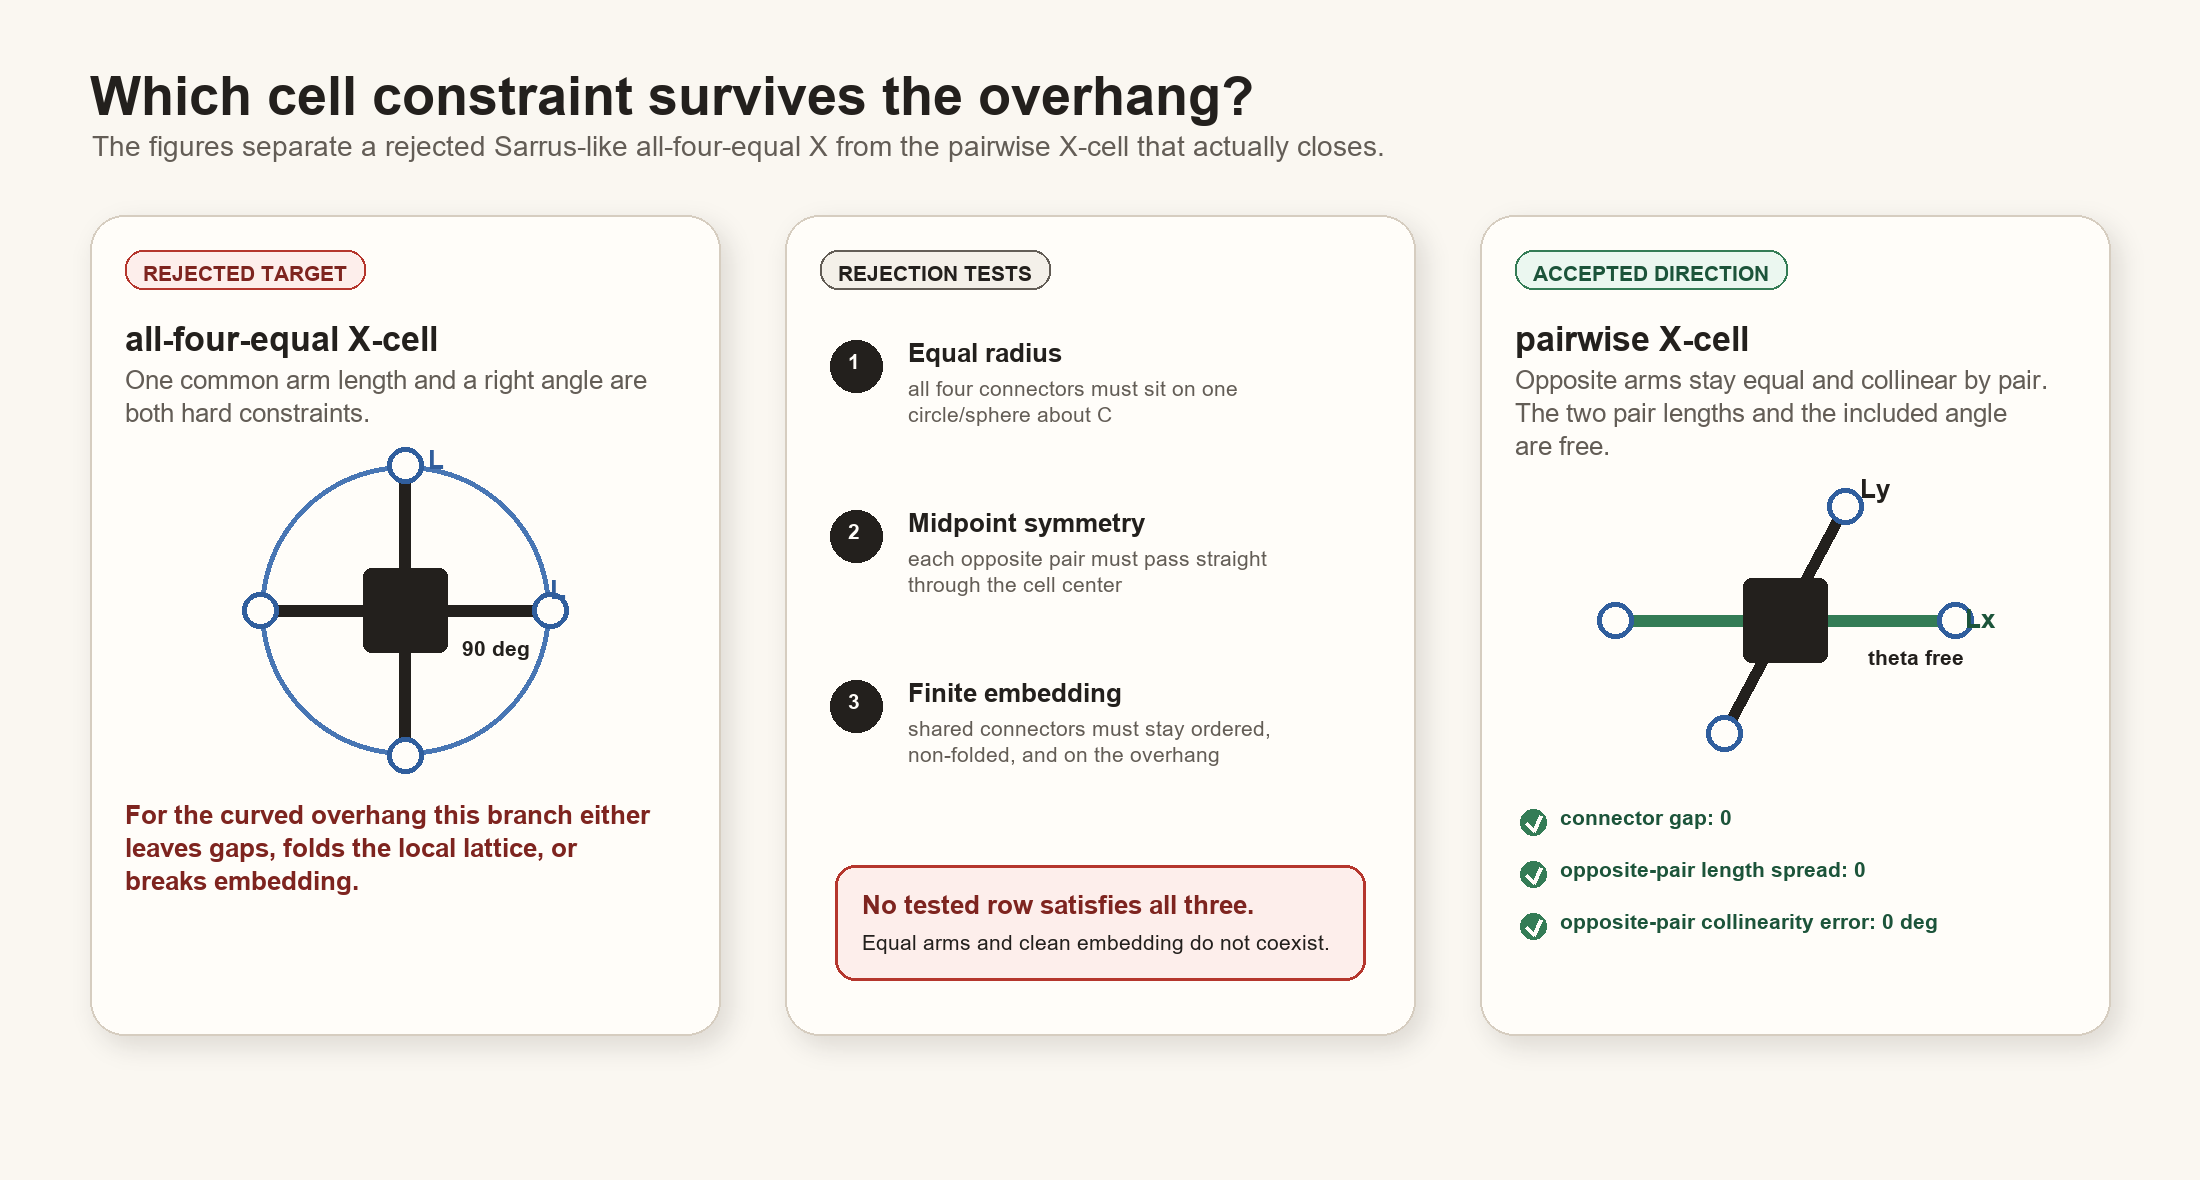
\includegraphics[width=0.93\linewidth]{constraint-contract-summary.png}
\caption{Mechanism contract inherited from the constraint proof and updated in the current renderer. WaveVis should preserve exact shared contact, one-center cells, and two-cell connector joints on adjacent-center spans rather than hiding infeasible geometry behind filler surfaces or a connector-ID count.}
\end{figure}

\section{Rendering modes}

WaveVis has three product views:
\begin{itemize}
  \item \textbf{3D/isometric view} shows the full rectangular array in perspective.
  \item \textbf{Side view} is a camera view of the full three-dimensional render from the side and must show the curl.
  \item \textbf{Top view} shows the full square plan sheet with localized interior deformation and catches terminal caps, triangular fans, wedges, or cropped-patch regressions.
\end{itemize}

The view contract matters because a side view can hide the curl if lateral geometry forms a wall over the open underside. In that case the correct fix is to reshape the three-dimensional surface so the lateral envelope follows the wave contour and fades out, not to switch the side view into a profile-only debug output or hide the wall.

\section{Verification gates}

The generator should be checked with both numeric and visual gates. Numeric checks are not sufficient, but they catch repeated hard failures before visual review.

\begin{table}[H]
\centering
{\small
\begin{tabular}{Y{0.26\linewidth}Y{0.28\linewidth}Y{0.34\linewidth}}
\toprule
Gate & Measurement & Acceptance intent \\
\midrule
Perimeter flatness & \(\max_{\partial\Omega}\|p^*-p^0\|\). & Boundary displacement is zero or visually negligible. \\
Topology completeness & Expected node, edge, and quad counts. & Full rectangular sheet graph remains visible. \\
Connector closure & Edge endpoints meet their node coordinates. & No detached legs or fake bridges. \\
Lip curl & Crest-to-lip height gap, terminal slope, run gate, and cavity gate. & The lip curls down into a smooth tapered branch rather than ending as a hill, near-vertical chute, hooked tip, bowl, dimple, or cavity. \\
Span localization & Row-wise height profile across \(y\). & Center strong, sides faded; no swept tunnel. \\
Morph continuity & Residual between adjacent morph samples. & No sudden jumps or topology flips. \\
Slider isolation & Aligned geometries across position/steer/width changes. & Rigid controls stay rigid; width stays span-only. \\
Visual side check & Browser side view screenshot or direct render inspection. & Curl visible in the full side view. \\
Defect repair loop & Confirmed visible defects re-enter source repair. & Acknowledging dimples, pockets, walls, or missing curl is not a stopping state. \\
Terminal side-profile gate & Literal readable profile and sampled model side trace. & Before visual QA, reject any lower-branch re-rise, under-lip valley rebound, lower-branch backtrack, abrupt terminal angle jump, or steep visible terminal descent. \\
Startup URL parser & Covers all public and legacy slider aliases. & A shared verification URL cannot silently load a different height, overhang, lip dip, width, or smoothing state. \\
Paper figure hygiene & Every figure is a target reference, accepted mechanism proof, current accepted render, or labeled rejected diagnostic. & Internal overlays, stale screenshots, and profile-only traces cannot become authoritative paper evidence. \\
\bottomrule
\end{tabular}
}
\caption{Verification gates. A build passing TypeScript is not enough; WaveVis must pass the rendered outcome Alan actually uses.}
\end{table}

\subsection{Current regression command set}

The current source-level gate is:
\[
  \code{npm run check:geometry}
\]
which expands to:
\begin{quote}
\small
\code{node scripts/check-geometry-invariants.cjs}\\
\code{node scripts/check-inverse-sheet.cjs}
\end{quote}
The inverse-sheet checker compiles the TypeScript geometry into a temporary CommonJS module and then evaluates the default state, low/high lip dip, morph, position, steer, flat contribution, smoothing, width, lateral taper, bowl-pocket, side-render, and startup-URL cases. The geometry-invariant checker covers mechanism-level consistency.

The current acceptance evidence expected from \code{scripts/check-inverse-sheet.cjs} includes:
\begin{itemize}
  \item startup display defaults to \code{showSurface=true}, \code{showEdges=true}, \code{showNodes=true}, and \code{showHeatmap=false};
  \item rendered black-square cell count equals the full rectangular grid count \(4928\);
  \item rendered center-to-connector X leg segment count equals the expected connector-use count \(19400\);
  \item every interior X cell has exactly four legs from one black square body;
  \item rendered spherical connector-node count equals the expected adjacent connector count \(9700\);
  \item each physical connector has exactly two endpoint uses;
  \item maximum X connector endpoint gap is zero;
  \item maximum opposite-pair length spread is zero;
  \item maximum opposite-pair collinearity error is zero degrees;
  \item maximum opposite-center residual is zero;
  \item connector corridor drift is bounded as a diagnostic rather than used as the pass condition;
  \item \code{sourceUsesCollinearEqualPairConnectors=true};
  \item connected X-cell bodies stay close to the sampled wave surface rather than becoming a detached fake mechanism;
  \item no bowl-pocket count is reported for default, compact-user, and breaking-wide presets;
  \item the literal readable side trace, side/isometric readable profile, startup default, user morph half-lip case, and slider sweeps all pass the terminal and readable side-profile cavity blockers before browser screenshots are treated as useful evidence;
  \item \code{blockSurfaceBowlPockets} runs on the target grid before morphing and node emission, and the named \(79\)-case slider sweep reports empty \code{badCases} arrays for the side-cavity and surface-bowl gates;
  \item side-overhang aspect stays in the downturned-lip band after the supplied-line update: startup default aspect between \(1.35\) and \(3.05\), compact user morph case between \(1.45\) and \(3.15\), and both with reach-to-height between \(0.72\) and \(1.35\);
  \item broad open-curl lip stats keep open-throat, no-dimple, no-under-overhang-bite, no-backfold, and return-to-flat checks true;
  \item those lip stats allow a wide rounded cap and tucked nose instead of forcing the old vertical-chute proxy;
  \item slider robustness exits cleanly for the named acceptance sweeps, while printed diagnostic subcases can still expose unsupported-resolution or terminal-angle failures that must not be described as accepted visual states.
\end{itemize}

These checks are designed around Alan's repeated failures. If a future change removes one of these cases because it is inconvenient, that is a regression unless the PDF and source explain an intentional replacement gate that still catches the same failure.

\subsection{Rendered verification}

Numeric checks must be followed by rendered verification. The minimum visual pass is:
\begin{enumerate}
  \item render the exact user URL/preset, not a nearby default;
  \item check \code{Side}: full 3D side camera, visible curl, no profile-only substitution, no wall covering the open underside, and no dimple or dark pocket under the overhang;
  \item check \code{3D}: full-sheet perspective view, visible curl/overhang, localized center deformation, no swept tunnel, no hidden rows, and no underside bite hidden by the camera angle;
  \item check \code{Top}: the sheet should remain square while the interior footprint localizes toward the curl; it must not become a constant extruded strip, broad terminal cap, clipped patch, or large triangular fan;
  \item inspect cells/connectors at the curl for zig-zags, random long arms, detached legs, overlaps, or missing four-leg interior connectivity;
  \item check lower \code{lipDip} values as well as \(120^\circ\), because old low-lip cases became unstable even when max lip looked acceptable;
  \item check \code{morph}=0, 0.5, and 1 because half-morph repeatedly exposed mangled intermediate states.
\end{enumerate}

Screenshots are evidence only when they show the actual rendered canvas and the URL or visible controls identify the tested state. A screenshot of a nice profile line is not evidence that the full linkage array is correct.

\section{Build, deploy, and publication runbook}

\subsection{Local development}

Use the WaveVis app root:
\[
  \code{\_apps/wavevis.aolabs.io/}.
\]
Typical local commands are:
\begin{itemize}
  \item \code{npm run dev} to run the Vite development server;
  \item \code{npm run check:geometry} to run geometry and mechanism checks;
  \item \code{npm run build} to build the static app;
  \item \code{npm run deploy} to publish the app's own GitHub Pages branch.
\end{itemize}
Do not manually edit \code{dist}. Build it from source.

\subsection{Public fallback deployment}

The route Alan can reliably use is \code{https://aolabs.io/wavevis/}. That route is served from the AO Labs hub/fallback repository, not directly from the WaveVis app repository. Therefore a public WaveVis update requires two publication steps when the fallback route is the user-facing route:
\begin{enumerate}
  \item build and publish the WaveVis app;
  \item copy the built \code{dist} contents into \code{\_apps/aolabs-site/wavevis/};
  \item commit and push the AO Labs site mirror;
  \item verify that \code{https://aolabs.io/wavevis/} serves the new bundle hash and the rendered artifact.
\end{enumerate}
This is not optional. A source commit or WaveVis \code{gh-pages} deploy can still leave Alan looking at a stale \code{aolabs.io/wavevis/} bundle.

\subsection{Custom-domain boundary}

\code{https://wavevis.aolabs.io/} is the preferred branded route, but a hostname/certificate failure means it is not the verified artifact. The current Progress source separates \code{wavevis\_home} from \code{wavevis\_custom\_domain}. Keep them separate. Do not claim the custom subdomain is fixed until a fresh request verifies the certificate and body from that hostname.

\subsection{Progress logging}

After meaningful WaveVis work, write a Progress event before final response when practical. The event must include:
\begin{itemize}
  \item \code{source\_ids}: usually \code{wavevis\_home} and \code{wavevis\_custom\_domain};
  \item Alan's complaint/request;
  \item the issue being solved;
  \item the Codex change;
  \item the observed public source change;
  \item provenance: thread, commits, checks, screenshots, and deployment basis;
  \item uncertainty: exact match not proven, custom domain stale, or any unverified surface.
\end{itemize}
Progress does not automatically ingest every active Codex chat. If a future WaveVis chat uses this PDF and changes the app, it must still write the event itself.

\section{Current verified and open state}

This section is intentionally blunt so a future chat does not have to infer whether the system is finished.

\textbf{Verified current facts on July 1, 2026:}
\begin{itemize}
  \item The reliable public route is \code{https://aolabs.io/wavevis/}; the preferred HTTPS subdomain remains a separate certificate/live-route check.
  \item The Inverse Sheet tab is the first/default option; Double-Layer Sarrus is secondary.
  \item The public PDF route is \code{/wavevis/proofs/wavevis-system-architecture.pdf}.
  \item Side, Front, Top, and 3D are product view modes. Side is a full three-dimensional sheet view, not a profile-only debug trace.
  \item The current source tree contains the one-center four-leg X mechanism renderer, black square cell-body renderer, spherical connector-node renderer, and the geometry checkers that measure those invariants, but the inverse-sheet source-level visible-mechanism contract is not closed.
  \item Candidate876 fails the local inverse-sheet checker \pathcode{scripts/check-inverse-sheet.cjs} because the visible mechanism source contract reports \pathcode{sourceUsesConnectedXMechanism=false}. The measured numeric connector occupancy still reports two-use physical connector nodes in the current checker output, but the source contract failure blocks a full pass. This is a current mechanism verification boundary, not a reference-match fact.
  \item Candidate876 passes local \code{npm run build}; the built bundle is in \code{dist/}.
  \item Candidate876 browser captures exist in:
  \begin{quote}\footnotesize
  \pathcode{_verification/}\\
  \pathcode{browser-20260701-}\\
  \pathcode{candidate876-broader-terminal/}
  \end{quote}
  The folder contains side, front, top, isometric, and forced mechanism-on views.
  \item The wrong internal reference-overlay figure, the rejected black side-profile line, and irrelevant stills have been removed from the paper figure sequence.
\end{itemize}

\textbf{Open state that blocks completion:}
\begin{itemize}
  \item Candidate876 was previously source/build/PDF/live-route checked as a baseline, but it is not a publication-accepted reference match after the July 1, 2026 pointy-profile complaint.
  \item Candidate785, Candidate841 through Candidate875, and Candidate898 through Candidate903 are not final accepted states. They remain rejected or superseded diagnostics.
  \item The current side profile is still too pointy relative to the accepted reference family, and the current isometric support-cone read still blocks an exact reference-match claim.
  \item Exact matching to the June 24 gridded reference, June 28 stage/cross-section reference, or retained ocean-curl photographs is not proven. The rejected black side-line drawing is not an acceptance target.
  \item This is a simulator and architecture record. It is not evidence that a physical lattice prototype has been fabricated or experimentally validated.
  \item If the live app, source, screenshots, Progress, or this PDF disagree, the current rendered artifact and source tree must be inspected and reconciled before any completion claim.
\end{itemize}

\section{Failure modes}

The most important failure classes are now explicit:
\begin{enumerate}
  \item \textbf{Swept barrel.} One side profile is dragged sideways at constant span. The result reads as a tunnel, roof, half-pipe, or bridge.
  \item \textbf{Side-wall cover.} The lip may exist in a center profile, but full side view shows a wall covering the open underside.
  \item \textbf{Straight chute.} The crest drops nearly vertically to a flat shelf instead of curling forward and under.
  \item \textbf{Blob or lump.} Excess smoothing or broad support creates a mound with no wave identity.
  \item \textbf{Top dent.} The outer crest has a kink or concave dent where a smooth radius is required.
  \item \textbf{Dimple, cavity, under-lip bite, or bowl.} The surface creates a pocket, pucker, enclosed hollow, under-overhang throat notch, or bowl-like depression rather than a plunging sheet.
  \item \textbf{Dangling terminal connection.} The side view avoids the old dimple metric but leaves a visible lower terminal tongue or foot under the lip. This still fails because the reference curl has a smooth open throat and a flat sheet return, not a small support hook that visually wires the lip to the ground.
  \item \textbf{Stale URL state.} A browser URL contains height, overhang, width, lipDip, or smoothing values, but startup ignores them and renders a different state.
  \item \textbf{Zig-zag linkage.} Neighboring legs alternate direction or length erratically.
  \item \textbf{Hidden mechanism.} Broken topology is ghosted, clipped, or replaced by a cosmetic surface.
  \item \textbf{Pointy surrogate target.} A clean black side line or internal contour is treated as the target even though it produces a pointy profile and does not define the gridded sheet, top footprint, front body, open throat, or visible mechanism.
  \item \textbf{Wrong paper evidence.} A stale overlay, profile trace, internal debug diagram, or rejected candidate screenshot appears as if it is a correct reference or accepted result.
  \item \textbf{Passive defect acknowledgement.} A visible problem is named in chat or recorded in this paper, but the generator and rendered artifact are not repaired and rechecked.
\end{enumerate}

The solution direction is to simplify the target field while strengthening the gates: localized smooth wave first, full array second, mechanism-clean render third. Complexity should be added only if it improves one of those outcomes without breaking the others.

\section{Materials and Methods}

The implementation source is the WaveVis React and TypeScript app~\cite{wavevis_source_2026}. The main geometry source is \code{src/latticeGeometry.ts}. The primary render source is \code{src/LatticeViewer3D.tsx}. Controls are declared in \code{src/TargetShapeControls.tsx}. Regression checks are run through \code{scripts/check-inverse-sheet.cjs}.

The model is deliberately written as an inspectable engineering simulator rather than a black-box optimizer. The validation style borrows from topology-optimization practice, where a compact code can still be valuable when its filters, constraints, and objective terms are explicit~\cite{sigmund_99line_2001,sigmund_maute_2013}; from linkage and compliant-mechanism design, where target motion is inseparable from topology, joint placement, actuator choice, and manufacturable compliance~\cite{coros_mechanical_characters_2013,thomaszewski_linkage_characters_2014,megaro_compliant_mechanisms_2017,sigmund_compliant_1997}; from deformation-programmed material and soft-robot design, where the local material or actuator rule controls the reachable shape space~\cite{bickel_deformation_materials_2010,rus_tolley_soft_robots_2015}; from inflatable and auxetic inverse design, where a desired three-dimensional target must be produced by a planar pattern or cell field rather than by a decorative surface~\cite{skouras_designing_inflatable_2014,konakovic_auxetic_2016,panetta_surface_inflatables_2021}; and from mechanical metamaterials, where local cell rules can create global deformation modes but can also produce unintended instabilities if the cell rule is not made explicit~\cite{bertoldi_instability_2010,coulais_textured_2016,kadic_3d_metamaterials_2019}. WaveVis currently encodes those lessons as hard source gates rather than as a mature continuous optimizer.

The public app serves a static build. The architecture PDF is placed in the public proofs directory as \code{wavevis-system-architecture.pdf} and linked from the WaveVis control headers. The old connector proof remains a source artifact for the mechanism decision, but the visible paper action now points to this architecture record because the current work is broader than connector assignment.

\section{Discussion}

The main design lesson is that WaveVis cannot be corrected by tuning only the side profile. The user-facing failure was three-dimensional: side walls, swept tubes, missing full-array linkages, broken side-view semantics, pointy front fins, and zig-zag legs. The architecture therefore now uses a single curated target contract rather than a manual editor contract. The sheet generator is responsible for creating a localized breaking-wave displacement field with lateral fade, boundary preservation, topology completeness, and a visible curled lip.

This distinction also clarifies future work. If the simulator produces a good center profile but a bad side view, the profile is only evidence that the curve exists somewhere. The real artifact still fails if the full three-dimensional render hides the curl or reads as an extrusion. Similarly, if the mesh is clean but the wave looks like a low mound, the mechanism is not enough. Both the shape and the linkage must be correct.

A newer lesson is that defect naming is not progress by itself. If a rendered state shows dimples, under-overhang pockets, side walls, or a missing curl, the correct workflow is source repair, geometry-check update, rendered screenshot verification, and public-bundle verification. The current checks name this directly through \code{noVisibleDimplePocket} and \code{readableSideProfileCavityBlock}: the lip must remain an open downturned branch with visible clearance and a return that advances into the flat sheet instead of folding into a pucker or dark throat bite. The same source-of-truth rule applies to URL state. Several correction screenshots used URLs that carried explicit height, overhang, width, lipDip, and smoothing values; ignoring those parameters caused the page to render a different geometry than the requested test state. The startup parser is now part of validation through \code{startupUrlParamCoverage}. The architecture record is useful only if it changes the generator, state loader, and acceptance loop; it cannot substitute for a corrected human-facing WaveVis render.

\section{Acknowledgements}

This record was written to reduce repeated handoff burden during WaveVis development. The repeated complaints about side walls, missing cells, zig-zag legs, profile-view confusion, and swept-barrel geometry are treated as acceptance criteria rather than optional polish notes.

\section{Funding}

No external funding is claimed in this system architecture record.

\section{Author contributions}

Alan N. Pham defined the target artifact, accepted and rejected visual states, and the mechanism constraints. Codex generated this architecture record from the current WaveVis source and the active development contract.

\section{Competing interests}

The author declares no competing interests for this internal architecture record.

\section{Data availability}

The source data for this record is the WaveVis source tree, the accepted June 24 gridded reference family, the June 28 stage/cross-section reference, the retained ocean-curl references copied into the proof figure set, the local proof diagrams, rejected-candidate verification folders, and the current simulator behavior. The rejected black side-profile line is recorded only as a failure class, not as accepted source data. The public PDF is served with the WaveVis static app.

\section{Code availability}

The relevant implementation files are \code{src/latticeGeometry.ts}, \code{src/LatticeViewer3D.tsx}, \code{src/TargetShapeControls.tsx}, and \code{scripts/check-inverse-sheet.cjs} in the WaveVis app repository.

\section{Additional information}

This document supersedes the old header link to the narrow connector-contact constraint proof as the primary public WaveVis PDF. The connector proof remains an implementation reference for mechanism feasibility, but the current public artifact needs the broader system architecture and outcome-verification contract.

\section{References}

\printbibliography[heading=none]

\end{document}

